\documentclass[11pt]{llncs}

\def\makeitbig{%
\setlength{\textwidth}{15.9cm}%
\setlength{\oddsidemargin}{.01cm}%
\setlength{\evensidemargin}{.01cm}%
\setlength{\textheight}{21.5cm}%
\setlength{\topmargin}{-.25cm}%
\setlength{\headheight}{.7cm}%
\leftmargini 20pt     \leftmarginii 20pt%
\leftmarginiii 20pt   \leftmarginiv 20pt%
\leftmarginv 12pt     \leftmarginvi 12pt%
\pagestyle{myheadings}}%

\makeitbig

\usepackage{algorithmicx}
\usepackage[english]{babel}
\usepackage[utf8]{inputenc}
\usepackage{amsmath, amsfonts, amssymb, graphicx, rotating, epsfig}
\usepackage{verbatim}
\usepackage{algorithm}
\usepackage[noend]{algpseudocode}
\usepackage{url}
\usepackage{tikz}
\usepackage{tabularx,multirow}
\usepackage{xspace}
\usepackage{booktabs}

\newcommand*\Let[2]{\State #1 $\gets$ #2}
%\algrenewcommand\alglinenumber[1]{
%    {\sf\footnotesize\addfontfeatures{Colour=888888,Numbers=Monospaced}#1}}


\newcommand{\sig}{{\sf $($Gene\-rate, Sign, Verify$)$} }
\newcommand{\ignore}[1]{}
\newcommand{\btr}{{\tt btrsync}}
\newcommand{\rsy}{{\tt rsync}}
\newcommand{\abs}[1]{\left|#1\right|}
\newcommand{\Cov}[0]{\mbox{Cov}}
\newcommand{\Var}[0]{\mbox{Var}}
\newcommand{\xor}[0]{\oplus}
\newcommand{\rmu}[0]{\mbox{RM}}
\newcommand{\Prob}[1]{{\Pr\left[\,{#1}\,\right]}}
\newcommand{\EE}[1]{{\mathbb{E}\left[{#1}\right]}}
\newcommand{\Oapp}{\ensuremath{\tilde{O}}}

\newcommand{\btrsync}{\texttt{btrsync}\xspace}
\newcommand{\rsync}{\texttt{rsync}\xspace}

\newcommand{\comm}[1]{\marginpar{%
\vskip-\baselineskip %raise the marginpar a bit
\raggedright\footnotesize
\itshape\hrule\smallskip#1\par\smallskip\hrule}}
\setlength{\marginparwidth}{2cm}

\usepackage{hyperref}

\begin{document}

\title{When File Synchronization Meets Number Theory}

\author{Antoine Amarilli \and Fabrice Ben Hamouda \and Florian Bourse \and\\
Robin Morisset \and David Naccache \and Pablo Rauzy}

\institute{
\'{E}cole normale sup\'{e}rieure, D\'{e}partement d'informatique \\
   45, rue d'Ulm, {\sc f}-75230, Paris Cedex 05, France.\\
   \email{surname.name@ens.fr} (except for \email{fabrice.ben.hamouda@ens.fr})
}

\maketitle

\begin{abstract}
This work revisits {\sl set reconciliation}, a problem consisting in
synchronizing two multisets while minimizing the amount of data transmitted. We
propose a new number theoretic reconciliation protocol called ``Divide \&
Factor''. Like prior proposals, our protocol in optimal in terms of asymptotic
transmission complexity. Nonetheless, this new protocol offers interesting
parameter trade-offs resulting in experimentally measured {\sl constant-factor}
transmission gains over the popular software \rsync. Reconciliation experiments
show that the new protocol usually transmits less data than \rsync at the
expense of lengthier calculations.\smallskip
\end{abstract}

\section{Introduction}
This work revisits {\sl set reconciliation}, a problem consisting in
synchronizing two multisets while minimizing the amount of data transmitted. Set
reconciliation arises in many practical situations, the most typical of which is
certainly incremental backups performed over a slow network link.\smallskip

Set reconciliation has already several efficient and elegant solutions. For
instance, \cite{PSRec} presents a particularly interesting reconciliation
protocol whose computational and communication complexities are linear in the
number of differences between the reconciled multisets, which mathches the
obvious lower bound.\smallskip

We refer the reader to \cite{PSRec,Mins1,Whats} (to quote a few references) for more on the problem's history and its existing solutions.\smallskip

This article proposes a new reconciliation protocol based on number theory. In
terms of asymptotic  transmission complexity, the proposed procedure reaches
optimality, like prior proposals. Nonetheless, the new protocols offer interesting parameter trade-offs resulting in experimentally measured {\sl constant-factor} gains over the popular software \rsync.\smallskip

We observed during most of our reconciliation experiments that the new protocol transmitted less bytes than \rsync\ but required lengthier calculations.\smallskip

Beyond these practical concerns the mathematical ideas underlying this work seem new and interesting as such.

TODO: announce the structure of the rest of the paper.

\section{``Divide \& Factor'' Set Reconciliation}

\subsection{Problem Definition and Notations}

\underline{O}scar possesses an \underline{o}ld version of a directory
$\mathfrak{D}$ that he wishes to update. \underline{N}eil has the
\underline{n}ew, up-to-date version $\mathfrak{D}'$: $\mathfrak{D}$ and
$\mathfrak{D}'$ can differ both in their files and in their tree structure.
Oscar wishes to obtain knowledge about $\mathfrak{D}'$ but wishes to {\sl
exchange as little data as possible} during the synchronization
process.\smallskip

To tackle this problem we separate the {\sl ``what''} from the {\sl ``where''}
and disregard the relative position of files. We represent $\mathfrak{D}$ as a
multiset of files which we denote as $\mathfrak{F}=\{F_0,\ldots,F_{n}\}$, and
likewise represent $\mathfrak{D'}$ as
$\mathfrak{F}'=\{F'_0,\ldots,F'_{n'}\}$.\smallskip

Let $t_0$ be the number of discrepancies between $\mathfrak{F}$ and $\mathfrak{F}'$ that Oscar wishes to learn, {\sl i.e.}:

$$t_0=\#\mathfrak{F}+\#\mathfrak{F}'-2 \#\left(\mathfrak{F} \bigcap \mathfrak{F}'\right)=\#\left(\mathfrak{F}\bigcup\mathfrak{F}'\right)-\#\left(\mathfrak{F}\bigcap\mathfrak{F}'\right)$$

Given a file $F$, we denote by $\mbox{{\tt Hash}}(F)$ its image by a
collision-resistant hash function such as SHA-1. Let $\mbox{{\tt
HashPrime}}(F)$\footnote{We discuss the design of \mbox{{\tt HashPrime}} in
Appendix~\ref{sec:hashprime}.} be a function hashing files (uniformly) into
primes smaller than $2^u$. [TODO(antoine): what is the definition of $u$, is it
something like ``there exists $u$ such that HashPrime hashes to primes smaller
than $2^u$''?]. Define the shorthand notations: $h_i=\mbox{{\tt
HashPrime}}(F_i)$ and $h'_i=\mbox{{\tt HashPrime}}(F'_i)$.\smallskip

\subsection{Description of the Basic Exchanges}
\label{basic}

The quantity $t_0$ is unknown to Oscar and Neil. However, in our protocol, Oscar
and Neil will assume that $t_0$ is smaller than some $t$ and attempt to perform
synchronization. If they are right, synchronization will succeed; if they are
wrong, they will transmit more information and try again, as will be explained
later.

We generate a prime $p$ such that:

\begin{equation}
\label{equp}
2^{2ut+1} \leq p < 2^{2ut+2}
\end{equation}

Given $\mathfrak{F}$, Oscar generates and sends to Neil the redundancy:

$$
c=\prod_{F_i\in \mathfrak{F}} \mbox{{\tt HashPrime}}(F_i)=\prod_{i=1}^n h_i \bmod p
$$

Neil computes:\smallskip

$$c'=\prod_{F'_i\in \mathfrak{F'}} \mbox{{\tt HashPrime}}(F'_i)=\prod_{i=1}^{n'} h'_i \bmod p{~~~\mbox{and}~~~}s=\frac{c'}{c} \bmod p$$

Using \cite{vallee} the integer $s$ can be written as:
$$s=\frac{a}{b} \bmod p{\mbox{~where the~}G_i\mbox{~denote files and~}}
\left\{
\begin{array}{lcr}
a & =&  \prod\limits_{G_i \in \mathfrak{F}'\wedge G_i \not\in\mathfrak{F}} \mbox{{\tt HashPrime}}(G_i) \\
\\
b & = & \prod\limits_{G_i \not\in\mathfrak{F}' \wedge G_i \in\mathfrak{F}} \mbox{{\tt HashPrime}}(G_i)
\end{array}
\right.
$$

Note that if our assumption $t_0 \leq t$ is correct $\mathfrak{F}$ and
$\mathfrak{F}'$ differ by at most $t$ elements and $a$ and $b$ are strictly less
than $2^{ut}$. Theorem \ref{theo} (see \cite{cryptorational}) guarantees $a$ and
$b$ can be efficiently recovered from $s$: this problem is known as the {\sl
Rational Number Reconstruction} \cite{pan2004rational,wang2003acceleration} and
is typically solved using Gauss' algorithm for finding the shortest vector in a
bi-dimensional lattice \cite{vallee}.

\begin{theorem}
\label{theo}
Let $a,b \in {\mathbb Z}$ such that $-A \leq a \leq A$ and $0<b \leq B$. Let $p>2AB$ be a prime and $s=a b^{-1} \mod p$.
Then $a,b$ can be recovered from $A,B,s,p$ in polynomial time.
\end{theorem}

Taking $A=B=2^{ut}-1$, (\ref{equp}) implies that $2AB<p$. Moreover, $0 \leq a \leq A$ and $0 <b \leq B$. Thus Oscar can
recover $a$ and $b$ from $s$ in polynomial time. By testing the divisibility of $a$ and $b$ by the $h_i$ and the $h'_i$, Neil and Oscar can
deterministically identify the discrepancies between $\mathfrak{F}$ and $\mathfrak{F}'$ and settle them.\smallskip

Formally, this is done as follows:\smallskip

\begin{center}
\begin{tabular}{|lcl|}\hline
~~{\bf Oscar}                       &                                                      &   {\bf Neil}~\\
~~computes $c$&                                                      &\\
                                   &~~{{\LARGE $\stackrel{c}{\longrightarrow}$}}~~        &   \\
                                   &                                                      &computes $a,b$~\\
                                   &                                                      &if $a$ doesn't factor into a product of $h'_i$s~\\
                                   &                                                      &~~~~~~then output $\bot$ and halt~\\
                                   &                                                      &~~~~~~else let $\mathfrak{S}=\{F'_i \mbox{~s.t.~} a \bmod h'_i =0\}$~~\\
                                   &~~{\LARGE $\stackrel{\mathfrak{S},b}{\longleftarrow}$}&\\
~~deletes files s.t. $b \bmod h_i =0$&                                                      &\\
~~adds $\mathfrak{S}$ to the disk    &                                                      &\\\hline
\end{tabular}
\end{center}

As we have just seen, the ``output $\bot$ and halt'' protocol interruption should never occur if indeed $t_0 \leq t$. However, a file synchronization procedure that works {\sl only} for a limited number of differences is not really useful in practice. Section~\ref{insuf} explains how to extend the protocol even when the number of differences exceeds $t$, the informational capacity of the modulus $p$.[TODO(antoine): I'm not I understand why if $t$ is too small we cannot have that $a$ factors into a product of $h'_i$s even though the protocol has actually failed and $b$ is not what we expect. Will this really \emph{never} occur, or is it very unlikely?]

\subsection{The Case of Insufficient Information}
\label{insuf}
To extend the protocol to an arbitrary $t_0$, Oscar and Neil agree on an infinite set of primes $p_1,p_2,\ldots$ As long as the protocol fails, Neil will keep accumulating information about the difference between $\mathfrak{F}$ and $\mathfrak{F}'$ as shown in Appendix~\ref{sec:extended}. Note that no information is lost and that the transmitted modular knowledge about the difference adds up until it reaches a threshold sufficient to reconcile $\mathfrak{F}$ and $\mathfrak{F}'$.\smallskip

\section{Transmission Complexity}

This section explores two strategies to reduce the size of $p$ and hence improve transmission by {\sl constant factors} (from an asymptotic communication standpoint, improvements cannot be expected as the protocol already transmits information proportional to $t$, the difference to settle). [TODO(antoine): This claim is not entirely obvious to me. I think it would be worthwhile to do some simple accounting to give the size of everything that is transferred so that everyone can see that we are indeed linear in the size of the symmetric difference.]

\subsection{Probabilistic Decoding: Reducing $p$}

Generate a prime $p$ about twice shorter than the $p$ recommended in section \ref{basic}, namely:
\begin{equation}
\label{eqnewp}
2^{ut+w-1}<p \leq 2^{ut+w}
\end{equation}

where $w \geq 1$ is some small integer (say $w=50$). Let $\eta=\max(n,n')$. The new redundancy $c$ is calculated as previously and is hence also approximately twice smaller. Namely:

$$s=\frac{a}{b} \bmod p \mbox{~and~}
\left\{
\begin{array}{lcr}
a & =&  \prod\limits_{G_i \in \mathfrak{F}'\wedge G_i \not\in\mathfrak{F}} \mbox{{\tt HashPrime}}(G_i) \\
\\
b & = & \prod\limits_{G_i \not\in\mathfrak{F}' \wedge G_i \in\mathfrak{F}} \mbox{{\tt HashPrime}}(G_i)
\end{array}
\right.
$$

and since there are at most $t$ differences, we must have:
\begin{equation}
\label{eqab}
a b \leq 2^{ut}
\end{equation}

By opposition to section \ref{basic} we do not have a fixed bound for $a$ and $b$ anymore; equation (\ref{eqab}) only provides a bound for the {\sl product} $a b$. Therefore, we define a sequence of at most $\lceil ut/w \rceil+1$ couples of bounds:

$$\left(A_i,B_i\right)=\left(2^{wi},\left\lfloor \frac{p-1}{2^{wi+1}} \right\rfloor\right)\mbox{~~where~~}B_i>1\mbox{~~and~~}\forall i>0,~2 A_i B_i<p$$

Equations (\ref{eqnewp}) and (\ref{eqab}) imply that there must exist at least one index $i$ such that $0 \leq a \leq A_i$ and $0 <b \leq B_i$. Then using Theorem \ref{theo}, given $(A_i,B_i,p,s)$ one can recover $(a,b)$, and hence the difference between $\mathfrak{F}$ and $\mathfrak{F}'$.\smallskip

The problem is that (unlike section \ref{basic}) we have no guarantee that such an $(a,b)$ is unique. Namely, we could (in theory) stumble over an $(a',b')\neq (a,b)$ satisfying (\ref{eqab}) for some index $i' \neq i$. We expect this to happen with negligible probability (that we do not try to estimate here) when $w$ is large enough, but this makes the modified protocol heuristic only. [TODO(antoine): Si je comprends bien, vous améliorez la complexité, mais en supposant que les choses se passent bien (et vous dites que c'est très probablement le cas). J'ai l'impression que c'est quand même un peu malhonnête de ne pas avoir un résultat sur l'\emph{espérance} de la quantité d'information à transmettre, en prenant aussi en compte les cas où les choses se passent mal ; ou bien, si on ne peut pas avoir de tel résultat, il faudrait avouer clairement qu'on conjecture juste que c'est meilleur en moyenne. Non ?] \smallskip

\subsection{The File Laundry: Reducing $u$}

What happens if we brutally shorten $u$ in the basic Divide \& Factor protocol?\smallskip

As expected by the birthday paradox, we should start seeing collisions. Let us analyze the statistics governing the appearance of collisions.

Consider $\mbox{{\tt HashPrime}}$ as a random function from $\{0,1\}^*$ to $\{0,\dots,2^u-1\}$. Let $X_i$ be the random variable:

$$
X_i =
\left\{
\begin{array}{lcl}
1 & ~~~~&  \mbox{if file $F_i$ collides with another file.}\\
\\
0 & ~~~~&  \mbox{otherwise.}
\end{array}
\right.
$$

Clearly, we have $\Prob{X_i = 1} \le \frac{\eta -1}{2^u}$.
The average number of colliding files is hence:
\[ \EE{\sum_{i=0}^{\eta-1} X_i} \le \sum_{i=0}^{\eta-1} \frac{\eta -1}{2^u} = \frac{\eta (\eta - 1)}{2^u} \]

For instance, for $\eta=10^6$ files and 32-bit digests, the expected number of colliding files is less than $233$.\smallskip

However, it is important to note that a collision can only yield a {\sl false positive}, and never a {\sl false negative}. In other words, while a collision may obliviate a difference\footnote{{\sl e.g.} make the parties blind to the difference between {\tt index.htm} and {\tt iexplore.exe}.} a collision will never create a nonexistent difference {\sl ex nihilo}.\smallskip

Thus, it suffices to replace $\mbox{{\tt HashPrime}}(F)$ by a diversified $\mbox{{\tt HashPrime}}(k|F)$ to quickly filter-out file differences by repeating the protocol for $k=1,2,\ldots$ At each iteration the parties will detect new files and new deletions, fix these and ``launder'' again the remaining multisets.\smallskip

Assume that the diversified $\mbox{{\tt HashPrime}}(k|F)$'s are random and independent. To understand why the probability that a stubborn file persists colliding decreases exponentially with the number of iterations $k$, assume that $\eta$ remains invariant between iterations and define the following random variables:\smallskip

$$
\begin{array}{rcl}
X^{\ell}_i & = &
\left\{
\begin{array}{lcl}
1 & ~~~~&  \mbox{if file $F_i$ collides with another file during iteration $\ell$.}\\
\\
0 & ~~~~&  \mbox{otherwise.}
\end{array}
\right.\\
\\
Y_i = \prod_{\ell=1}^k X^{\ell}_i & = &
\left\{
\begin{array}{lcl}
1 & ~~~~&  \mbox{if file $F_i$ collides with another file during the $k$ first protocol iterations.}\\
\\
0 & ~~~~&  \mbox{otherwise.}
\end{array}
\right.
\end{array}$$

By independence, we have:

 \[ \Prob{Y_i = 1} = \prod_{\ell=1}^k \Prob{X^{\ell}_i = 1} = \Prob{X^1_i = 1} \dots \Prob{X^k_i = 1} \le \left( \frac{\eta -1}{2^u} \right)^k \]
Therefore the average number of colliding files is:
\[
 \EE{\sum_{i=0}^{\eta-1} Y_i} \le \sum_{i=0}^{\eta-1} \left( \frac{\eta -1}{2^u} \right)^k =  \eta \left(\frac{\eta - 1}{2^u}\right)^k
\]

And the probability that at least one false positive will survive $k$ rounds is:

\[
\epsilon_k \le \eta \left(\frac{\eta - 1}{2^u}\right)^k
\]

For the previously considered instance\footnote{$\eta=10^6$,$u=32$.} we get $\epsilon_2 \le 5.43\%$ and $\epsilon_3 \le 2 \cdot 10^{-3}\%$.

\subsubsection{A more refined (but somewhat technical) analysis.} As mentioned previously, the parties can remove the files confirmed as different during iteration $k$ and work during iteration $k+1$ only with common and colliding files. Now, the only collisions that can fool round $k$, are the collisions of file-pairs $(F_i,F_j)$ such that $F_i$ and $F_j$ have both already collided during {\sl all the previous iterations}\footnote{Note that we \underline{do not} require that $F_i$ and $F_j$ repeatedly collide {\sl which each other}. {\sl e.g.} we may witness during the first round $\hbar_{1,u}(F_1)=\hbar_{1,u}(F_2)$ and $\hbar_{1,u}(F_3)=\hbar_{1,u}(F_4)$ while during the second round $\hbar_{2,u}(F_1)=\hbar_{2,u}(F_4)$ and $\hbar_{2,u}(F_2)=\hbar_{2,u}(F_3)$.}. We call such collisions ``masquerade balls''. Define the two random variables:

\begin{align*}
Z^\ell_i &=
\left\{
\begin{array}{lcl}
1 & ~~~~&  \mbox{if $F_i$ participated in masquerade balls during all $\ell$ first protocol iterations.}\\
\\
0 & ~~~~&  \mbox{otherwise.}
\end{array}
\right. \\
X^{\ell}_{i,j} &=
\left\{
\begin{array}{lcl}
1 & ~~~~&  \mbox{if files $F_i$ and $F_j$ collide during iteration $\ell$.}\\
\\
0 & ~~~~&  \mbox{otherwise.}
\end{array}
\right.
\end{align*}
\comm{Inclure ici image du bal masque}

Set $Z^0_i = 1$ and write $p_\ell = \Prob{Z^{\ell-1}_{i} = 1 \text{ and } Z^{\ell-1}_{j} = 1} $ for all $\ell$ and $i \neq j$.
For $k \ge 1$, we have:
\begin{align*}
\Prob{Z^k_i=1} &= \Prob{\exists j\neq i \text{, } X^k_{i,j} = 1 \text{, } Z^{k-1}_{i} = 1  \text{ and } Z^{\ell-1}_{j} = 1}  \\
&\le \sum_{j=0, j\neq i}^{\eta-1} \Prob{X^{k-1}_{i,j} = 1} \Prob{Z^{k-1}_{i} = 1 \text{ and } Z^{k-1}_{j} = 1}  \\
&\le \frac{\eta-1}{2^u} p_{k-1}
\end{align*}
Furthermore $p_0 = 1$ and
\begin{align*}
p_\ell &= \Prob{X^{\ell}_0 = X^{\ell}_1 \text{, } Z^{\ell}_{0} = 1 \text{ and } Z^{\ell}_{1} = 1}
  + \Prob{X^{\ell}_0 \neq X^{\ell}_1 \text{, } Z^{\ell}_{0} = 1 \text{ and } Z^{\ell}_{1} = 1} \\
&\le \Prob{X^{\ell}_0 = X^{\ell}_1 \text{, } Z^{\ell-1}_{0} = 1 \text{ and } Z^{\ell-1}_{1} = 1} \\
  &\quad+ \sum_{i \ge 2, j \ge 2} \Prob{X^\ell_{0,i} = 1 \text{, } X^\ell_{1,j} = 1 \text{, } Z^{\ell-1}_{0} = 1 \text{ and } Z^{\ell-1}_{1} = 1} \\
&= \Prob{X^{\ell}_0 = X^{\ell}_1} \Prob{Z^{\ell-1}_{0} = 1 \text{ and } Z^{\ell-1}_{1} = 1} \\
  &\quad+ \sum_{i \ge 2, j \ge 2} \Prob{X^\ell_{0,i} = 1} \Prob{X^\ell_{1,j} = 1} \Prob{Z^{\ell-1}_{0} = 1 \text{ and } Z^{\ell-1}_{1} = 1} \\
&\le \frac{1}{2^u} p_{\ell-1} + \frac{(\eta-2)^2}{2^{2u}} p_{\ell-1} = p_{\ell-1}\left(\frac{1}{2^u}  + \frac{(\eta-2)^2}{2^{2u}}\right)
\end{align*}
hence:
\[ p_\ell \le \left( \frac{1}{2^u} + \frac{(\eta-2)^2}{2^{2u}} \right)^\ell, \]
and
\[ \Prob{Z^\ell_i=1} \le \left( \frac{1}{2^u} + \frac{(\eta-2)^2}{2^{2u}} \right)^{k-1} \]
And finally, the survival probability of at least one false positive after $k$ iterations satisfies:
\[
\epsilon'_k \le \frac{\eta(\eta-1)}{2^u} \left( \frac{1}{2^u} + \frac{(\eta-2)^2}{2^{2u}} \right)^{k-1}
\]

For $(\eta=10^6,u=32,k=2)$, we get $\epsilon'_2 \le 0.013\%$.\smallskip

\subsubsection{How to select $u$?}
% 
For a fixed $k$, $\epsilon'_k$ decreases as $u$ grows. For a fixed $u$, $\epsilon'_k$ also decreases as $k$ grows. Transmission, however, grows with both $u$ (bigger digests) and $k$ (more iterations). We write for the sake of clarity: $\epsilon'_k = \epsilon'_{k,u,\eta}$.\smallskip

Fix $\eta$. Note that the number of bits transmitted per iteration ($\simeq 3ut$), is proportional to $u$. This yields an expected transmission complexity bound $T_{u,\eta}$ such that:\smallskip

\[T_{u,\eta} \propto u \sum_{k=1}^{\infty} k \cdot \epsilon'_{k,u,\eta}=
\frac{u \eta\left(\eta-1\right)}{2^u} \sum_{k=1}^{\infty} k \left( \frac{1}{2^u} + \frac{\left(\eta-2\right)^2}{2^{2u}} \right)^{k-1}=
\frac{u \eta\left(\eta-1\right) 8^u}{\left(2^u-4^u+\left(\eta-2\right)^2\right)^2}\]

Dropping the proportionality factor $\eta\left(\eta-1\right)$, neglecting $2^u \ll 2^{2u}$ and approximating $(\eta-2)\simeq\eta$, we can optimize the function:

\[
\phi_\eta(u)=\frac{u \cdot 8^u}{\left(4^u-\eta^2\right)^2}
\]

$\phi_{10^6}(u)$ admits an optimum for $u=19$.

\subsubsection{Note:} The previous analysis is a rough approximation, in particular:

\begin{itemize}
\item We consider $u$-bit prime digests while $u$-bit strings contain only about $2^u/u$ primes.\smallskip

\item In all our probability calculations $\eta$ can be replaced by the total number of differences $t$. It is reasonable to assume that in most {\sl practical} settings $t \ll \eta$, but extreme instances where $t\sim\eta$ can sometimes be encountered as well.\smallskip

\item We used a fixed $u$ in all rounds. Nothing forbids using a different $u_k$ at each iteration\footnote{...or even fine-tuning the $u_k$s adaptively, as a function of the laundry's effect on the progressively reconciliated multisets.}.

\item Our analysis treated $t$ as a constant, but large $t$ values increase $p$ and hence the number of potential files detected as different per iteration - an effect disregarded in our analysis.
\end{itemize}

Given that, after all, optimization may only result in constant-factor improvements, we suggest to optimize $t$ and $u$ experimentally, {\sl e.g.} using the open source program \btrsync\ developed by the authors ({\sl cf.} section  \ref{program}).

\subsection{How to Stop a Probabilistic Washing Machine?} We now combine both optimizations and assume that $\ell$ laundry rounds are necessary for completing some given reconciliation task using a half-sized $p$. By opposition to section \ref{basic}, confirming correct protocol termination is now non-trivial.\smallskip

Let the round failure probability\footnote{{\sl i.e.} that probability that a round resulted in an $(a',b')\neq (a,b)$ satisfying equation (\ref{eqab}).} be some function $\upsilon(w)$ (that we did not estimate). If $w$ is kept small (for efficiency reasons), the probability $\left(1-\upsilon(w)\right)^{\ell}$ that the protocol will properly terminate may dangerously drift away from one.\smallskip

If $v$ of $\ell+v$ rounds fail, Oscar needs to solve a problem called {\sl Chinese Remaindering With Errors}:\smallskip

\begin{problem}{\sl (Chinese Remaindering With Errors Problem: {\sc crwep} \cite{phong}).} Given as input integers $v$, $B$ and $\ell+v$ points $(s_1,p_1),\ldots,(s_{\ell+v},p_{\ell+v})\in \mathbb{N}^2$ where the $p_i$'s are coprime, output all numbers $0 \leq s < B$ such that $s \equiv s_i \bmod p_i$ for at least $v$ values of $i$.
\end{problem}

We refer the reader to \cite{phong} for more on this problem, which is beyond the scope of this article. Boneh \cite{boneh} provides a polynomial-time algorithm for solving the {\sc crwep} under certain conditions satisfied by our setting.\smallskip

To detect that reconciliation succeeded, Neil will send to Oscar $\mbox{{\tt Hash}}(\mathfrak{F}')$ as soon as the interaction starts. As long as Oscar's {\sc crwep} resolution does not result in a state matching $\mbox{{\tt Hash}}(\mathfrak{F}')$, the parties will continue the interaction.

\section{Computational Complexity}

Let $\mu(k)$ be the time required to multiply two $k$-bit numbers\footnote{We suppose that $\forall k,k', \mu(k+k') \ge \mu(k) + \mu(k')$.}.
The modular division of two $k$-bit numbers and the reduction of $2k$-bit number modulo a $k$-bit number are known to cost $\Oapp(\mu(k))$ \cite{burnikel1998fast}.\smallskip

For na\"{i}ve ({\sl i.e.} convolutive) algorithms $\mu(k) = O(k^2)$, but using {\sc fft} multiplication strategies \cite{schonhage1971schnelle}, $\mu(k) = \Oapp(k)$. {\sc fft} is experimentally faster than convolutive methods for $k \sim 10^6$ and on. For such sizes, in packages such as {\sf gmp}, division and modular reduction also run in $\Oapp(\mu(k))$. Given that $p \sim 2^{ut}$, we get the following complexity analysis:

\comm{"reduction also run in $\Oapp(\mu(k))$"}

\begin{table}
  \begin{tabularx}{\textwidth}{lXp{1.2cm}p{2.3cm}p{1.2cm}p{2.3cm}}\toprule
{\bf \hfill Entity \hfill \null} & {\bf \hfill Computation \hfill \null} &
    \multicolumn{4}{c}{{\bf Complexity expressed in $\Oapp$ of}} \\\midrule
Both  & redundancies $c$ and $c'$                                        & $n \cdot \mu(u t)$  & na\"{i}ve product & $n u t$  & using {\sc fft}             \\
Oscar & $s = c' / c \bmod p$                                             & $\mu(u t)$    & na\"{i}ve inversion& $u t$    & using {\sc fft}               \\
Oscar & $a,b$ such that $s = a / b \bmod p$                              & $(u t)^2$   & na\"{i}ve ext. {\sc gcd} & $\mu(u t)$ &  using \cite{pan2004rational,wang2003acceleration} \\
Both  & factorization of $a$ (resp. $b$) by modular reductions           & $n \cdot \mu(u t)$  & na\"{i}ve reduction & $n u t$  & using {\sc fft}             \\
      & {\bf Overwhelming complexity:}                                   &
    \multicolumn{2}{c}{$\max((u t)^2,n \cdot \mu(ut))$ }    &
    \multicolumn{2}{c}{$n u t$}              \\\bottomrule
  \end{tabularx}
  \caption{Global Protocol Complexity. In practice $\max((u t)^2,n \cdot \mu(ut))=n(u t)^2$ because $(u t)^2 \ll n \cdot \mu(ut)=n(u t)^2$}
  \label{tab:workload}
\end{table}


\subsection{Improvements}

The overwhelming complexities of the computations of $(c,c')$ and of the factorizations can be reduced to $\Oapp(\frac{n}{t} \mu(u t))$ using convolutive methods and to $\Oapp(n u)$ with {\sc fft} \cite{schonhage1971schnelle}. To simplify explanations, assume that $t=2^\tau$ is a power of two dividing $n$.

The idea is the following: group $h_i$s by subsets of $t$ elements and compute the product of each such subset in $\mathbb{N}$.
\[ H_j = \prod_{i=j t}^{j t + t - 1} h_i. \]

Each $H_j$ can be computed in $\Oapp(\mu(u t))$ using the standard product tree method described in Algorithm~\ref{alg:prod-tree} (for $j=0$) and illustrated in Figure~\ref{fig:prod-tree}.
And all these $\frac{n}{t}$ products can be computed in $\Oapp(\frac{n}{t} \mu(u t))$. Then, one can compute $c$ by multiplying the $H_j$ modulo $p$, which costs $\Oapp(\frac{n}{t} \mu(u t))$.

\newpage

\begin{figure}[t]
\centering
\centerline{
\begin{turn}{90}
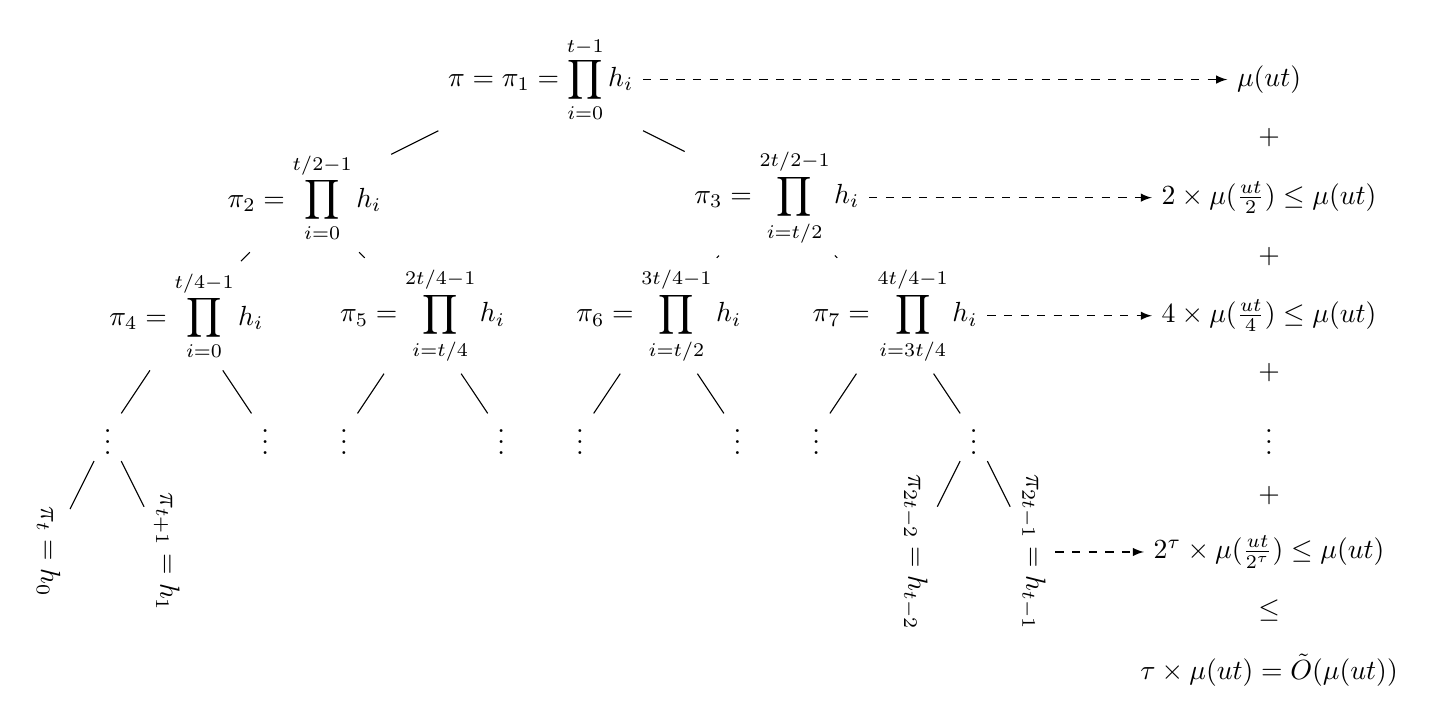
\begin{tikzpicture}[level/.style={sibling distance=60mm/#1}]
\node (z){$\displaystyle \pi=\pi_1=\prod_{i=0}^{t-1} h_i$}
  child {node (a) {$\displaystyle \pi_2=\prod_{i=0}^{t/2-1} h_i$}
    child {node (b) {$\displaystyle \pi_4=\prod_{i=0}^{t/4-1} h_i$}
      child {node {$\vdots$}
        child {node (d) {\begin{turn}{270}{$\displaystyle \pi_t=h_0$}\end{turn}}}
        child {node (e) {\begin{turn}{270}{$\displaystyle \pi_{t+1}=h_1$}\end{turn}}}
      }
      child {node {$\vdots$}}
    }
    child {node (g) {$\displaystyle \pi_5=\prod_{i=t/4}^{2t/4-1} h_i$}
      child {node {$\vdots$}}
      child {node {$\vdots$}}
    }
  }
  child {node (j) {$\displaystyle \pi_3=\prod_{i=t/2}^{2t/2-1} h_i$}
    child {node (k) {$\displaystyle \pi_6=\prod_{i=t/2}^{3t/4-1} h_i$}
      child {node {$\vdots$}}
      child {node {$\vdots$}}
    }
    child {node (l) {$\displaystyle \pi_7=\prod_{i=3t/4}^{4t/4-1} h_i$}
      child {node {$\vdots$}}
      child {node (c){$\vdots$}
        child {node (o) {\begin{turn}{270}{$\displaystyle \pi_{2t-2}=h_{t-2}$}\end{turn}}}
        child {node (p) {\begin{turn}{270}{$\displaystyle \pi_{2t-1}=h_{t-1}$}\end{turn}}
%
%
          child [grow=right] {node (qe) {} edge from parent[draw=none]
            child [grow=right] {node (q) {$2^\tau \times \mu(\frac{ut}{2^\tau}) \le \mu(u t)$} edge from parent[draw=none]
            child [grow=up] {node (r) {$\vdots$} edge from parent[draw=none]
            child [grow=up] {node (s) {$4\times\mu(\frac{u t}4) \le \mu(u t)$} edge from parent[draw=none]
            child [grow=up] {node (t) {$2\times\mu(\frac{u t}2) \le \mu(u t)$} edge from parent[draw=none]
            child [grow=up] {node (u) {$\mu(u t)$} edge from parent[draw=none]}
          }}}
          child [grow=down] {node (v) {$\tau \times \mu(u t) = \Oapp(\mu(u t))$}edge from parent[draw=none]}
            }
          }
        }
    }
  }
};
\path (q) -- (r) node [midway] {+};
\path (s) -- (r) node [midway] {+};
\path (s) -- (t) node [midway] {+};
\draw[->,>=latex,dashed] (l) to (s);
\path (t) -- (u) node [midway] {+};
\draw[->,>=latex,dashed] (z) to (u);
\draw[->,>=latex,dashed] (j) to (t);
\draw[->,>=latex,dashed] (p) to (q);
\path (q) -- (v) node [midway] {$\displaystyle \le$};
\end{tikzpicture}
\end{turn}
}
\caption{Product Tree}\label{fig:prod-tree}
\end{figure}

\newpage

\begin{algorithm}
\newcommand{\vstart}{\ensuremath{\mathrm{start}}}
\newcommand{\vmid}{\ensuremath{\mathrm{mid}}}
\newcommand{\vend}{\ensuremath{\mathrm{end}}}
\begin{algorithmic}[1]
\Require{the set $h_i$}
\Ensure{$\pi = \pi_1 = \prod_0^{t-1} h_i$, and $\pi_i$ for $i \in \{1,\dots,2t-1\}$ as in Figure~\ref{fig:prod-tree}}
\State $\pi \gets $ array of size $t$
\Function{prodTree}{$i$,$\vstart$,$\vend$}
  \If{$\vstart = \vend$}
    \State \Return $1$
  \ElsIf{$\vstart+1 = \vend$}
    \State \Return $h_{\mbox{\tiny \vstart}}$
  \Else
    \State $\vmid \gets \lfloor \frac{\vstart+\vend}{2} \rfloor$
    \State $\pi_{2i} \gets $\Call{prodTree}{$2i$,$\vstart$,$\vmid$}
    \State $\pi_{2i+1} \gets $\Call{prodTree}{$2i+1$,$\vmid$,$\vend$}
    \State \Return $\pi_{2i} \times \pi_{2i+1}$
  \EndIf
\EndFunction
\State $\pi_1 \gets $\Call{prodTree}{$1,0,t$}
\end{algorithmic}
\caption{Product Tree Algorithm}\label{alg:prod-tree}
\end{algorithm}

The same technique applies to factorization\footnote{We explain the process with $a$, this is applicable {\sl ne variatur} to $b$ as well.}, but with a slight {\sl caveat}.\smallskip

After computing the tree product, we can compute the residues of $a$ modulo $H_0$. 
Then we can compute the residues of $a \mod H_0$ modulo the two children $\pi_2$ and $\pi_3$ of $H_0 = \pi_1$ in the product tree (depicted in Figure~\ref{fig:prod-tree}), and so on. Intuitively, we descend the product tree doing modulo reduction. At the end ({\sl i.e.}, as we reach the leaves), we obtain the residues of $a$ modulo each of the $h_i$ ($i \in \{0,\dots,t-1\}$). This is described in Algorithm \ref{fig:div-prod-tree} and illustrated in Figure \ref{fig:div-prod-tree}. 
We can use the same method for the tree product associated to any $H_j$, and so we can get the residues of $a$ modulo each of the $h_i$ ($i \in \{jt,\dots,jt+t-1\}$) for any $j$, {\sl i.e.}, $a$ modulo each of the $h_i$ for any $i$.
Complexity is $\Oapp(\mu(u t))$ for each $j$, summing-up to a total complexity of $\Oapp(\frac{n}{t} \Oapp(\mu(u t)))$.

\newpage
\begin{figure}[t]
\centering
\centerline{
\begin{turn}{90}
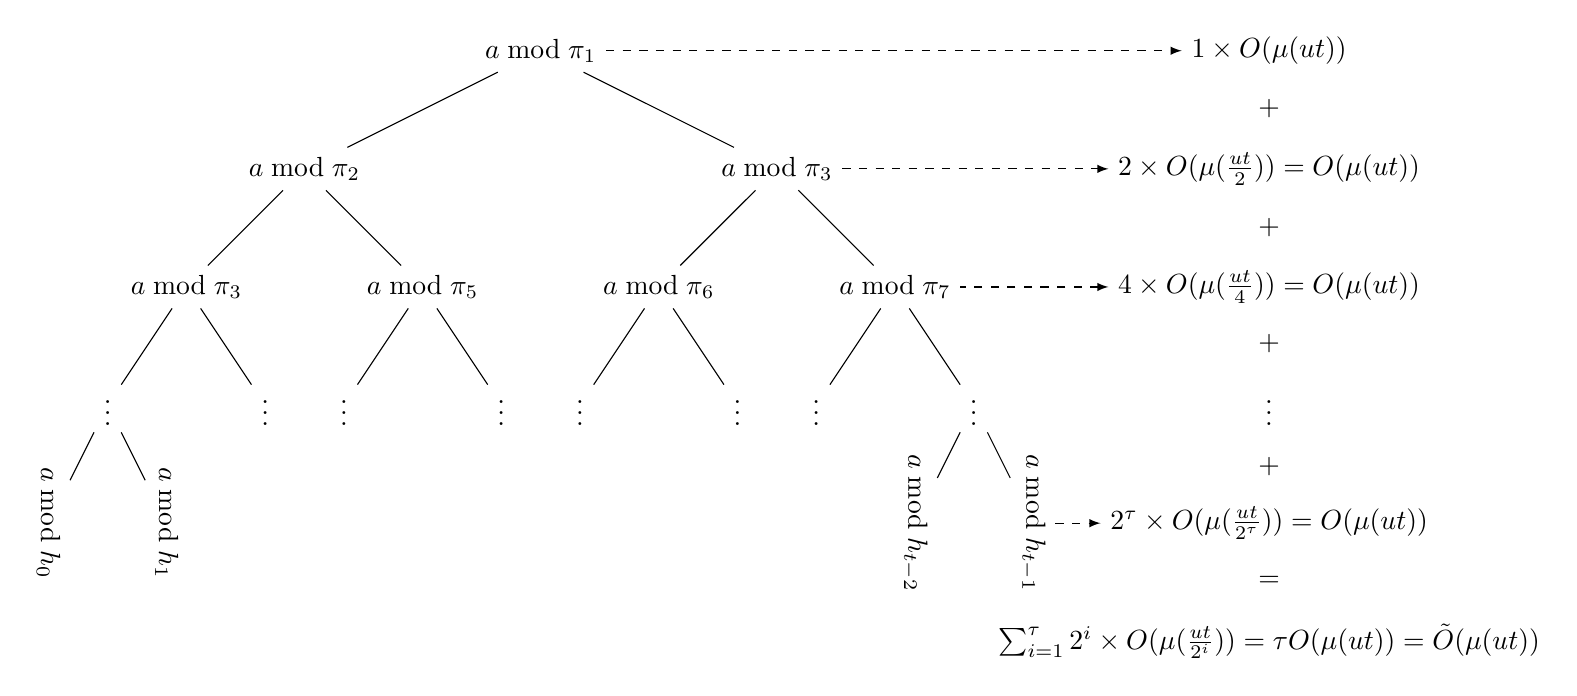
\begin{tikzpicture}[level/.style={sibling distance=60mm/#1}]
\node (z){$\displaystyle a \bmod \pi_1$}
  child {node (a) {$\displaystyle a \bmod \pi_2$}
    child {node (b) {$\displaystyle a \bmod \pi_3$}
      child {node {$\vdots$}
        child {node (d) {\begin{turn}{270}{$\displaystyle a \bmod h_{0}$}\end{turn}}}
        child {node (e) {\begin{turn}{270}{$\displaystyle a \bmod h_{1}$}\end{turn}}}
      }
      child {node {$\vdots$}}
    }
    child {node (g) {$\displaystyle a \bmod \pi_5$}
      child {node {$\vdots$}}
      child {node {$\vdots$}}
    }
  }
  child {node (j) {$\displaystyle a \bmod \pi_3$}
    child {node (k) {$\displaystyle a \bmod \pi_6$}
      child {node {$\vdots$}}
      child {node {$\vdots$}}
    }
    child {node (l) {$\displaystyle a \bmod \pi_7$}
      child {node {$\vdots$}}
      child {node (c){$\vdots$}
        child {node (o) {\begin{turn}{270}{$\displaystyle a \bmod h_{t-2}$}\end{turn}}}
        child {node (p) {\begin{turn}{270}{$\displaystyle a \bmod h_{t-1}$}\end{turn}}
%
%
          child [grow=right] {node (qe) {} edge from parent[draw=none]
            child [grow=right] {node (q) {$2^{\tau} \times O(\mu(\frac{ut}{2^{\tau}}))= O(\mu(u t))$} edge from parent[draw=none]
            child [grow=up] {node (r) {$\vdots$} edge from parent[draw=none]
            child [grow=up] {node (s) {$4 \times O(\mu(\frac{u t}4)) = O(\mu(u t))$} edge from parent[draw=none]
            child [grow=up] {node (t) {$2 \times O(\mu(\frac{u t}2)) = O(\mu(u t))$} edge from parent[draw=none]
            child [grow=up] {node (u) {$1 \times O(\mu(u t))$} edge from parent[draw=none]}
          }}}
          child [grow=down] {node (v) {$\sum_{i=1}^\tau 2^{i} \times O(\mu(\frac{ut}{2^i})) = \tau O(\mu(u t)) = \Oapp(\mu(u t))$}edge from parent[draw=none]}
            }
          }
        }
    }
  }
};
\path (q) -- (r) node [midway] {+};
\path (s) -- (r) node [midway] {+};
\path (s) -- (t) node [midway] {+};
\draw[<-,>=latex,dashed] (s) to (l);
\path (t) -- (u) node [midway] {+};
\draw[->,>=latex,dashed] (z) to (u);
\draw[->,>=latex,dashed] (j) to (t);
\draw[->,>=latex,dashed] (p) to (q);
\path (q) -- (v) node [midway] {$\displaystyle =$};
\end{tikzpicture}
\end{turn}}
\caption{Modular Reduction From Product Tree}\label{fig:div-prod-tree}
\end{figure}

\newpage

\begin{algorithm}
\newcommand{\vstart}{\ensuremath{\mathrm{start}}}
\newcommand{\vmid}{\ensuremath{\mathrm{mid}}}
\newcommand{\vend}{\ensuremath{\mathrm{end}}}
\begin{algorithmic}[1]
\Require{$a$ an integer, $\pi$ the product tree of Algorithm \ref{alg:prod-tree}}
\Ensure{$A[i] = a \bmod \pi_i$ for $i \in \{1,\dots,2t-1\}$, computed as in Figure \ref{alg:div-prod-tree}}
\State $A \gets $ array of size $t$
\Function{modTree}{$i$}
  \If{$i < 2t$}
    \State $A[i] \gets A[\lfloor i/2 \rfloor] \bmod \pi_i$
    \State \Call{modTree}{$2i$}
    \State \Call{modTree}{$2i+1$}
  \EndIf
\EndFunction
\State $A[1] \gets a \bmod \pi_1$
\State \Call{modTree}{$2$}
\State \Call{modTree}{$3$}
\end{algorithmic}
\caption{Division Using a Product Tree}\label{alg:div-prod-tree}
\end{algorithm}

\subsection{Adapting $p$}

Let $\mbox{{\tt Prime}}[i]$ denote the $i$-th prime\footnote{with $\mbox{{\tt Prime}}[1]=2$}. Besides conditions on size, the {\sl only} property required from $p$ is to be co-prime with all the $h_i$ and all the $h'_i$. We can hence consider the following variants:

\subsubsection{Variant 1:} Use a sequence of smooth $p_i$:

$$p_i=\prod_{j=r_i}^{r_{i+1}-1} \mbox{{\tt Prime}}[j]$$

Where the bounds $r_i$ are chosen to ensure that each $p_i$ has the proper size.

\subsubsection{Variant 2:} Define $p_i=\mbox{{\tt Prime}}[i]^{r_i}$ where the exponents $r_i$ are chosen to ensure that each $p_i$ has the proper size.

\subsubsection{Variant 3:} Progressively work modulo a long power of two. This variant, is probably the most efficient of all but somewhat complex to explain. We hence describe it in detail in Appendix \ref{powtwo}.

This variant is more delicate to explain as Where the exponents $r_i$ are chosen to ensure that each $p_i$ has the proper size.

\section{Implementation}
\label{program}

We implemented and benchmarked the method that we describe in the previous
sections. The implementation is called \btrsync, its source code is available
from~\cite{Robin}.

\smallskip

The program implements unidirectional synchronization, which is simpler to
understand. The implementation is divided in two subprograms: a shell script and
a Python program:

\subsection{The Shell Script}

The shell script sets up two instances of the Python program on Oscar and Neil
and establishes a bidirectional communication channel between them (materialized
by two Unix pipes between their standard input and output).

\subsection{The Python Program}

The Python program uses gmp to perform all the number theory operations required,
and performs the actual synchronization. It proceeds in two phases:

\subsubsection{Finding Different Files}

\begin{enumerate}
\item Compute the hashes of all files concatenated with their paths, type (folder/file), and permissions (not supported yet).
\item Implement the protocol proposed in Section \ref{} [add here a reference to the appropriate section in the paper] with input data coming from stdin and output data going to stdout.
\end{enumerate}

More precisely:
[TODO(antoine): isn't there going to be some overlap between this section and the description of the protocol in Appendix~\ref{sec:extended}? I feel we should explain the protocol elsewhere and only give implementation details here.]
\begin{itemize}
\item Oscar sends it product of hashes modulo a first prime number $p_1$.
\item Neil receives the product, divides by its own product of hashes, reconstructs the fraction modulo $p_1$ [can we elaborate more on what happens here? which functions in GMP are used to do the reconstruction?] and checks if he can factor the denominator using his hashes base. If he can, he stops and sends the numerator and the list of tuples (path, type, hash of content of the file) corresponding to the denominator's factors. Otherwise he sends "None" [is this the ASCII string "None"? if not what does he send precisely?].
\item If Neil sent "None", Oscar computes the product of hashes modulo another prime $p_2$, sends it... CRT mechanism... [can we elaborate more on what happens here? which functions in GMP are used to do the CRT?]
\item If Neil sent the numerator and a list of tuples, then Oscar factors the numerator over his own hash values. Now each party (Neil, Oscar) knows precisely the list of files (path + type + hash of content) that differs from the over party.
\end{itemize}

[please structure the following:]\smallskip

2. synchronize all the stuff [this is not an expression we can use in a paper...]. This part is not completely optimized.\smallskip

We just remove all folders Oscar should not have and create new folders.\smallskip

Then we remove all files Oscar should not have and synchronize using rsync the last files.\smallskip

We could check for move (since we have the list of hash of contents of files) and do moves locally.\smallskip

We can even try to detect moves of complete subtrees...\smallskip

\subsection{Move Resolution Algorithm}

To reproduce the structure of Oscar on Neil, we have a list of file moves to
apply. Sadly, it is not straightforward to apply the moves, because, if we take
a file to move, its destination might be blocked, either because a file already
exists (we want to move $a$ to $b$, $b$ already exists), or because a folder
cannot be created (we want to move $a$ to $b/c$, $b$ already exists but is a
file and not a folder). Note that for a move operation $a \rightarrow b$, there
is at most one file blocking the location $b$: we will call it the
\emph{blocker}.

If the blocker is not present on Oscar, then we can just delete it. However, if
it exists, then we might need to move it somewhere else before we solve the move
we are interested in. This move itself might have a blocker, and so on. It seems
that we just need to continue until we reach a move which has no blocker or
where the blocker can be deleted, but we can get caught in a cycle: if we must
move $a$ to $b$, $b$ to $c$ and $c$ to $a$, then we will not be able to perform
the operations without using a temporary location.

How can we perform the moves? A simple way would be to move each file to a
unique temporary location and then rearrange files to our liking: however, this
performs many unnecessary moves and could lead to problems if the program is
interrupted. We can do something more clever by performing a decomposition in
strongly connected components of the \emph{move graph} (with one vertex per file
and one edge per move operation going from to the file to its blocker or to its
destination if no blocker exists). The computation of the SCC decomposition is
simplified by the observation that because two files being moved to the same
destination must be equal, we can only keep one arbitrary in-edge per node, and
look at the graph pruned in this fashion: its nodes have in-degree at most one,
so the strongly connected components are either single nodes or cycles. Once the
SCC decomposition is known, the moves can be applied by applying each SCC in a
bottom-up fashion, an SCC's moves being solved either trivially (for single
files) or using one intermediate location (for cycles).

The detailed algorithm is implemented as two mutually recursive functions and
presented as Algorithm~\ref{alg:moves}.

% TODO check this algo
\begin{algorithm}
  \caption{Perform Moves}
  \label{alg:moves}
  \begin{algorithmic}[1]
    \Require{$\mathfrak{D}$ is a dictionary where $\mathfrak{D}[f]$ denotes the intended destinations of $f$}
    \Statex
    \Let{$M$}{[]}
    \Let{$T$}{[]}
    \For{$f$ in $\mathfrak{D}$'s keys}
      \Let{$M[f]$}{not\_done}
    \EndFor
    \Function{unblock\_copy}{$f, t$}
      \If{$t$ is blocked by some $b$}
        \If{$b$ is not in $\mathfrak{D}$'s keys}
          \State unlink($b$) \Comment{We don't need $b$}
        \Else
          \State \Call{resolve}{$b$} \Comment{Take care of $b$ and make it go away}
        \EndIf
      \EndIf
      \If{$T[f]$ was set}
        \Let{$f$}{$T[f]$}
      \EndIf
      \State copy($f$, $d$)
    \EndFunction
    \Function{resolve}{$f$}
      \If{$M[f] =$ done}
        \State \Return \Comment{Already managed by another in-edge}
      \EndIf
      \If{$M[f] =$ doing}
        \Let{$T[f]$}{mktemp()}
        \State move($f$, $T[f]$)
        \Let{$M[f]$}{done}
        \State \Return \Comment{We found a loop, moved $f$ out of the way}
      \EndIf
      \Let{$M[f]$}{doing}
      \For{$d \in \mathfrak{D}[f]$}
        \If{$d \neq f$}
          \State unblock\_copy($f$, $d$) \Comment{Perform all the moves}
        \EndIf
      \EndFor
      \If{$f \notin \mathfrak{D}[f]$ and $T[f]$ was not set}
        \State unlink($f$)
      \EndIf
      \If{$T[f]$ was set}
        \State unlink($T[f]$)
      \EndIf
    \EndFunction

    \For{$f$ in $\mathfrak{D}$'s keys}
      \State \Call{resolve}{$f$}
    \EndFor
  \end{algorithmic}
\end{algorithm}

An optimization implemented by \btrsync over the algorithm described here is to
move files instead of copying them and then removing the original file, because
moves are faster than copies on most filesystems as the OS does not need to copy
the actual file contents to perform them.

\subsection{Experimental Comparison to \rsync}

We compared \rsync\footnote{\rsync version 3.0.9, used both as a competitor to
benchmark against and as an underlying call in our own code.}
and our Divide \& Factor implementation called \btrsync under the following
experimental conditions:

\subsubsection{Test Directories:} The directories used for transmission and time
comparisons are described in Table~\ref{tab:benchdirec}.\smallskip

\subsubsection{Command-Line Options:} \rsync was called with the following options, for the reasons below:

$\blacktriangleright$ {\tt --delete} to delete existing files on Oscar which do
not exist on Neil like \btrsync does.\smallskip

$\blacktriangleright$ {\tt -I} to ensure that \rsync did not cheat by looking at file modification times (which \btrsync does not do).\smallskip

$\blacktriangleright$ {\tt --chmod="a=rx,u+w"} in an attempt to disable the transfer of file permissions (which \btrsync does not transfer). Although these settings ensure that \rsync does not need to transfer permissions, verbose logging suggests that it does transfer them anyway, so \rsync must lose a few bytes per file as compared to \btrsync for this reason.\smallskip

$\blacktriangleright$ {\tt -v} Transmission accounting was performed by calling \rsync with the {\tt -v} flag (which reports the number of sent and received bytes). For \btrsync we added a piece of code counting the amount of data transmitted during \btrsync's own negotiations.\smallskip

\subsubsection{Network Configuration:} The influence of the network on
performance can be approximated by the quantity of bandwidth. The benchmark was
done on a synchronization on two folders on the same host to try to account for
actual CPU time.

\subsubsection{Results:}

Results are given in Table~\ref{tab:results}. In general, \btrsync spent more
time than \rsync on computation (especially when the number of files is large,
which is typically seen on the experiments involving {\tt synthetic}).
Transmission results, however, turn out to be favorable to \btrsync.\smallskip

In the trivial experiments where either Oscar or Neil have no data at all,
\rsync outperforms \btrsync. This is especially visible when Neil has no data:
\rsync immediately notices that there is nothing to transfer, but \btrsync
engages in information transfers to determine the symmetric
difference.\smallskip

On non-trivial tasks, however, \btrsync outperforms \rsync. This is the case of
the {\tt synthetic} datasets, where \btrsync does not have to transfer
information about all unmodified files, and even more so in the case where there
are no modifications at all. For Firefox source code datasets, \btrsync saves a
very small amount of bandwidth, presumably because of unmodified files. For the
\btrsync source code dataset, we notice that \btrsync, unlike \rsync, was able
to detect the move and avoid retransferring the moved folder.

\section{Conclusion and Further Improvements}

\comm{Recopier de l'intro et adapter}

We strongly encourage the developer community to continue improving our open source software (that we called \btrsync).

\section{Acknowledgment}

The authors acknowledge Guillain Potron for his early involvement in this research work.\smallskip

\section{ToDo}

\begin{itemize}
\item @Fabrice @David: Je n'ai toujours pas compris si on a un argument clair
  pour dire qu'on est meilleur que \cite{Mins1}, du genre ``on prend en compte
  la taille des hachés, etc.'' Ce serait à mon avis beaucoup plus vendeur que de
  dire ``on fait pareil qu'eux, mais différemment'' et de parler d'``interesting
  parameter trade-offs''. :-)

\item @David: Je ne comprends pas pourquoi tu parles de ``constant-factor
  gains'' par rapport à rsync. Vu que rsync ne détecte absolument pas les moves,
  on n'a pas juste un facteur constant comme amélioration, enfin si ton problème
  c'est ''synchroniser un dataset de taille N avec un move d'un dossier de
  taille N/2'' on a une complexité asymptotique largement meilleure que rsync,
  je crois ?

\item Fix euclidean to Euclidean in reference 5.\smallskip

\item Merge two reference files rsynch and wagner.\smallskip

\item @Fabrice: Appendix B (je vais jeter un coup d'oeil la semaine prochaine)

\item @Fabrice: Fig. 1 pas clair, je pense qu'il faut mieux créer une notation mu gcd car en fait la FFT ne modifie que le mu... Et on pourrait plut\^ot indiquer dans ce tableau la complexité (avec mu et mu gcd) en utilisant l'optimisation décrite ou sans utiliser l'optimisation décrite). N'oublions pas de préciser que les temps des expériences d'Antoine comptent aussi le tirage des nombres premiers (qui doit \^etre négligeable peut-\^etre dans notre cas, je ne me rappelle plus...)

\item @Fabrice: Pour éviter le cas empty $\rightarrow$ source trop gros, on pourrait imaginer l'astuce suivante: si jamais Neil la taille de c est plus petite que la taille du produit des nombres premiers $p_1$...$p_n$ utilisés, Neil envoie un message pour l'indiquer, et on arr\^ete là le protocole. Et Oscar peut directement factoriser ce nombre envoyé...

\item @Fabrice: il faut discuter de la taille de la taille maximale des ``petits'' premiers utilisés pour les variantes de $p$ et montrer que cela n'enlève pas trop d'entropie pour les $h_i$. Encore une fois, je m'en occupe la semaine prochaine si besoin.

\item Refaire les expériences, vu que Fabrice a significativement amélioré les
  perfs. Du reste, autant les refaire en local...

\item Revoir l'intro.
\end{itemize}

\nocite{rsync}
\nocite{wagner}

\bibliographystyle{splncs03}
\bibliography{btrsync}

\begin{thebibliography}{30}

\bibitem{boneh} D. Boneh, {\sl Finding Smooth Integers in Short Intervals Using CRT Decoding}, Proceedings of the 32-nd Annual ACM Symposium on Theory of Computing, 2000, pp. 265--272.

\bibitem{phong} D. Bleichenbacher and Ph. Nguyen, Advances in Cryptology -- Proceedings of Eurocrypt'00, vol. 1807 of Lecture Notes in Computer Science, Springer-Verlag, pp. 53--69.

\bibitem{PSRec} Y. Minsky, A. Trachtenberg, {\sl Scalable Set Reconciliation}, 40th Annual Allerton Conference on Communications, Control and Computing, Monticello, IL, October 2002. A full version entitled {\sl Practical Set Reconciliation} can be downloaded from \url{http://ipsit.bu.edu/documents/BUTR2002-01.ps}

\bibitem{Mins1} Y. Minsky, A. Trachtenberg, R. Zippel, {\sl Set reconciliation with nearly optimal communication complexity}. IEEE Transactions on Information Theory, 49(9), 2003, pp. 2213–2218.

\bibitem{Whats} D. Eppstein, M. Goodrich, F. Uyeda, G. Varghese What's the difference?: efficient set reconciliation without prior context
ACM SIGCOMM Computer Communication Review - SIGCOMM '11, 41(4), 2011, pp. 218-229.

\bibitem{Robin} \url{https://github.com/RobinMorisset/Btrsync}

\end{thebibliography}

\appendix

\section{Extended Protocol}
\label{sec:extended}

\begin{center}
\begin{tabular}{lcl}\toprule
\multicolumn{3}{c}{{\sf First phase during which Neil amasses modular
information on the difference~~}} \\\midrule
~~{\bf Oscar}                      &                                                      &   {\bf Neil}~\\
                                   &                                                      &start the protocol with $p_1$~\\
                                   &~~{{\LARGE $\stackrel{c_1}{\longrightarrow}$}}~~      &   \\
                                   &                                                      &computes $a,b$ using $p_1$~\\
                                   &                                                      &if $a$ factors properly then go to {\sf Final Phase}\\
                                   &                                                      &~~~~~~else perform the protocol with $p_2$~~\\
                                   &~~{{\LARGE $\stackrel{c_2}{\longrightarrow}$}}~~      &   \\
                                   &                                                      &computes $c \bmod p_1 p_2=\mbox{CRT}_{p_1,p_2}(c_1,c_2)$~~\\
                                   &                                                      &computes $a,b$ using $p_1 p_2$~\\
                                   &                                                      &if $a$ factors properly then go to {\sf Final Phase}\\
                                   &                                                      &~~~~~~else perform the protocol with $p_3$~~\\
                                   &~~{{\LARGE $\stackrel{c_3}{\longrightarrow}$}}~~      &   \\
                                   &                                                      &computes $c \bmod p_1 p_2 p_3=\mbox{CRT}_{p_1,p_2,p_3}(c_1,c_2,c_3)$~~\\
                                   &                                                      &computes $a,b$ using $p_1 p_2 p_3$~\\
                                   &                                                      &if $a$ factors properly then go to {\sf Final Phase}\\
                                   &                                                      &~~~~~~else perform the protocol with $p_4$ ~~\\
                                   &                  $\vdots$
& \\\midrule
\multicolumn{3}{c}{{\sf Final Phase~~}} \\\midrule
                                   &                                                      & \\
                                   &                                                      &Let $\mathfrak{S}=\{F'_i \mbox{~s.t.~} a \bmod h'_i =0\}$~~\\
                                   &~~{\LARGE $\stackrel{\mathfrak{S},b}{\longleftarrow}$}&\\
                                   ~~deletes files s.t. $b \bmod h_i =0$&                                                      &\\
                                   ~~adds $\mathfrak{S}$ to the disk
                                   &
                                   &\\\bottomrule
\end{tabular}
\end{center}

Note that parties do not need to store the $p_i$'s in full. Indeed, the $p_i$s could be subsequent primes sharing their most significant bits. This reduces storage per prime to a very small additive constant $ \cong \mbox{ln}(p_i) \cong \mbox{ln}(2^{2tu+2}) \cong 1.39(tu+1)$ of about $\log_2(tu)$ bits.

\section{Power of Two Protocol}
\label{powtwo}

In this variant Oscar computes $c$ in $\mathbb{N}$:

$$
c=\prod_{F_i\in \mathfrak{F}} \mbox{{\tt HashPrime}}(F_i) = \prod_{i=1}^n h_i \in \mathbb{N}
$$

and considers $c=\bar{c}_{n-1}|\ldots|\bar{c}_2|\bar{c}_0$ as the concatenation of $n$ successive $u$-bit strings.

\begin{center}
\begin{tabular}{|lcl|}\hline
\multicolumn{3}{|c|}{{\sf First phase during which Neil amasses modular information on the difference~~}} \\\hline
~~{\bf Oscar}                      &                                                      &   {\bf Neil}~\\
~~computes $c\in \mathbb{N}$       &                                                      &\\
                                   &~~{{\LARGE $\stackrel{\bar{c}_0}{\longrightarrow}$}}~~&   \\
                                   &                                                      &computes $a,b$ modulo $2^u$~\\
                                   &                                                      &if $a$ factors properly then go to {\sf Final Phase}~~\\
                                   &                                                      &~~~~~~else request next chunk $\bar{c}_1$~~\\
                                   &~~{{\LARGE $\stackrel{\bar{c}_1}{\longrightarrow}$}}~~&   \\
                                   &                                                      &construct $c \bmod 2^{2u}=\bar{c}_1|\bar{c}_0$~~\\
                                   &                                                      &computes $a,b$ modulo $2^{2u}$~\\
                                   &                                                      &if $a$ factors properly then go to {\sf Final Phase}~~\\
                                   &                                                      &~~~~~~else request next chunk $\bar{c}_2$~~\\
                                   &~~{{\LARGE $\stackrel{\bar{c}_2}{\longrightarrow}$}}~~      &   \\
                                   &                                                      &construct $c\bmod 2^{3u}=\bar{c}_2|\bar{c}_1|\bar{c}_0$~~\\
                                   &                                                      &computes $a,b$ modulo $2^{3u}$~\\
                                   &                                                      &if $a$ factors properly then go to {\sf Final Phase}~~\\
                                   &                                                      &~~~~~~else request next chunk $\bar{c}_3$~~\\
                                   &                  $\vdots~(\mbox{~for~}\lambda \mbox{~rounds~})$    & \\\hline\hline
\multicolumn{3}{|c|}{{\sf Final Phase~~}} \\\hline
                                   &                                                      & \\
                                   &                                                      &Let $\mathfrak{S}=\{F'_i \mbox{~s.t.~} a \bmod 2^{\lambda u} =0\}$~~\\
                                   &~~{\LARGE $\stackrel{\mathfrak{S},b}{\longleftarrow}$}&\\
                                   ~~deletes files s.t. $b \bmod 2^{\lambda u} =0$&        &\\
                                   ~~adds $\mathfrak{S}$ to the disk    &                                                      &\\\hline
\end{tabular}
\end{center}

\section{Hashing Into Primes}
\label{sec:hashprime}
Hashing into primes is frequently needed in cryptography. A recommended implementation of $\mbox{{\tt HashPrime}}(F)$ is given in Algorithm \ref{alg:primes}. If $u$ is large enough ({\sl e.g.} $160$) one might sacrifice uniformity to avoid repeated file hashings using $\mbox{{\tt HashPrime}}(F)=\mbox{{\tt NextPrime}}(\mbox{{\tt Hash}}(F))$. Yet another acceleration option (that further destroys uniformity) consists in replacing $\mbox{{\tt NextPrime}}$ by the faster scanning Algorithm \ref{alg:scanprime} where $\alpha=2\times 3\times 5\times \cdots \times \mbox{{\tt Prime}}[d]$ is the product of the first primes until some rank $d$.

\begin{algorithm}
  \caption{Fast Nonuniform Hashing Into Primes}
  \label{alg:scanprime}
  \begin{algorithmic}[1]
  \State $h =\alpha \left\lfloor\frac{\mbox{{\tt Hash}}(F)}{\alpha}\right\rfloor+1$
\While{$h$ is composite}
\State $h = h-\alpha$
\EndWhile
\State \Return{$h$}
  \end{algorithmic}
\end{algorithm}

\begin{algorithm}
  \caption{Possible Implementation of $\mbox{{\tt HashPrime}}(F)$}
  \label{alg:primes}
  \begin{algorithmic}[1]
  \State $i=0$
\Repeat
\State $h = 2\cdot\mbox{{\tt Hash}}(F|i)+1$
\State $i = i+1$
\Until{$h$ is prime}
\State \Return{$h$}
  \end{algorithmic}
\end{algorithm}

\begin{table}
  \begin{tabular*}{\textwidth}{@{\extracolsep{\fill}}ll c c c c c c c c }
    \toprule
    \multicolumn{2}{c}{\bf Entities and Datasets} & \multicolumn{6}{c}{\bf Transmission (Bytes)} & \multicolumn{2}{c}{\bf Time (s)} \\
    \midrule {\bf \hfill Neil's $\mathfrak{F}'$ \hfill \null} & {\bf \hfill Oscar's $\mathfrak{F}$ \hfill \null}
    & {\bf TX$_r$} & {\bf RX$_r$} & {\bf TX$_b$} & {\bf RX$_b$} & {\bf abs} &
    {\bf rel} & {\bf t$_r$} & {\bf t$_b$} \\\midrule
    &&&&&&&&&\\[-1em]

    \texttt{source} & \texttt{empty} & 778311 & 1614 & 779517 & 10140 & 9732 & 1.0 & 0.1 & 0.4 \\
\texttt{empty} & \texttt{source} & 24 & 12 & 11927 & 5952 & 17843 & 496.6 & 0.1 & 0.4 \\
\texttt{empty} & \texttt{empty} & 24 & 12 & 19 & 30 & 13 & 1.4 & 0.0 & 0.3 \\
\texttt{synthetic} & \texttt{synthetic\_shuffled} & 54799 & 19012 & 7308 & 3417 & -63086 & 0.1 & 0.2 & 1.5 \\
\texttt{synthetic\_shuffled} & \texttt{synthetic} & 54407 & 18822 & 6822 & 3042 & -63365 & 0.1 & 0.2 & 0.8 \\
\texttt{synthetic} & \texttt{synthetic} & 54799 & 19012 & 327 & 30 & -73454 & 0.0 & 0.1 & 0.7 \\
\texttt{firefox-13.0.1} & \texttt{firefox-13.0} & 40998350 & 1187 & 39604079 & 3305 & -1392153 & 1.0 & 1.5 & 10.2 \\
\texttt{source\_moved} & \texttt{source} & 778176 & 1473 & 2757 & 1966 & -774926 & 0.0 & 0.1 & 0.6 \\

    \bottomrule

  \end{tabular*}

  \caption{Experimental results. The two first columns indicate the datasets,
    synchronization is performed \emph{from} Neil \emph{to} Oscar. RX and TX are
    received and sent byte counts, $r$ and $b$ are \rsync and \btrsync, we also
    provide the absolute difference in exchanged data $\textrm{abs} = \mathrm{TX}_b +
    \mathrm{RX}_b - \mathrm{TX}_r - \mathrm{RX}_r$ (positive when \btrsync
    transfers more data than \rsync) and the relative amount of data sent by
    \btrsync compared to \rsync $\mathrm{rel} = (\mathrm{TX}_b + \mathrm{RX}_b)
    / (\mathrm{TX}_r + \mathrm{RX}_r)$(over $100\%$ when \btrsync transfers more
  data than $\rsync$). The last two columns show timing results.}
  \label{tab:results}
\end{table}

\begin{table}
\begin{center}
\begin{tabular}{ll}\toprule
~~{\bf Directory}              ~~&~~{\bf Description}\\\midrule
~~{\tt synthetic}              ~~&~~A directory containing 1000 very small files containing~~\\
~~                             ~~&~~the numbers $1,2,\ldots,1000$. \\
~~{\tt synthetic\_shuffled}    ~~&~~{\tt synthetic} with:\\
                             ~~& ~~~~~10 deleted files\\
                             ~~& ~~~~~10 renamed files \\
                             ~~& ~~~~~10 modified files \\
~~{\tt source}                 ~~& ~~A snapshot of \btrsync's own source tree \\
~~{\tt source\_moved}          ~~& ~~{\tt source} with one big folder (a few megabits) renamed.~~\\
~~{\tt firefox-13.0}           ~~& ~~The source archive of Mozilla Firefox 13.0.\\
~~{\tt firefox-13.0.1}         ~~& ~~The source archive of Mozilla Firefox 13.0.1\\
~~{\tt empty}                  ~~& ~~An empty folder.\\\bottomrule
\end{tabular}\smallskip
  \caption{Test Directories.}
  \label{tab:benchdirec}
\end{center}
\end{table}



\end{document}
